\section{Evaluation of PREF for traffic splitting}

In order to well understand the requirements set for PREFLEX balancing by Path Re-Feedback, this section evaluates individually features and performance of PREF as a traffic splitting mode.  

Simulations were conducted using TEXCP framework to compare it with FLARE (Traffic Splitting technique used for FLARE).The two mechanisms were compared for two balancing approach: an equalization mode where the tendency is to send equal traffic over the available routes; and a simplified  version of TEXCP that balances the traffic based on path utilization but doesn't activate TEXCP congestion management mechanism.
 
\begin{figure}[h!]
\begin{center}
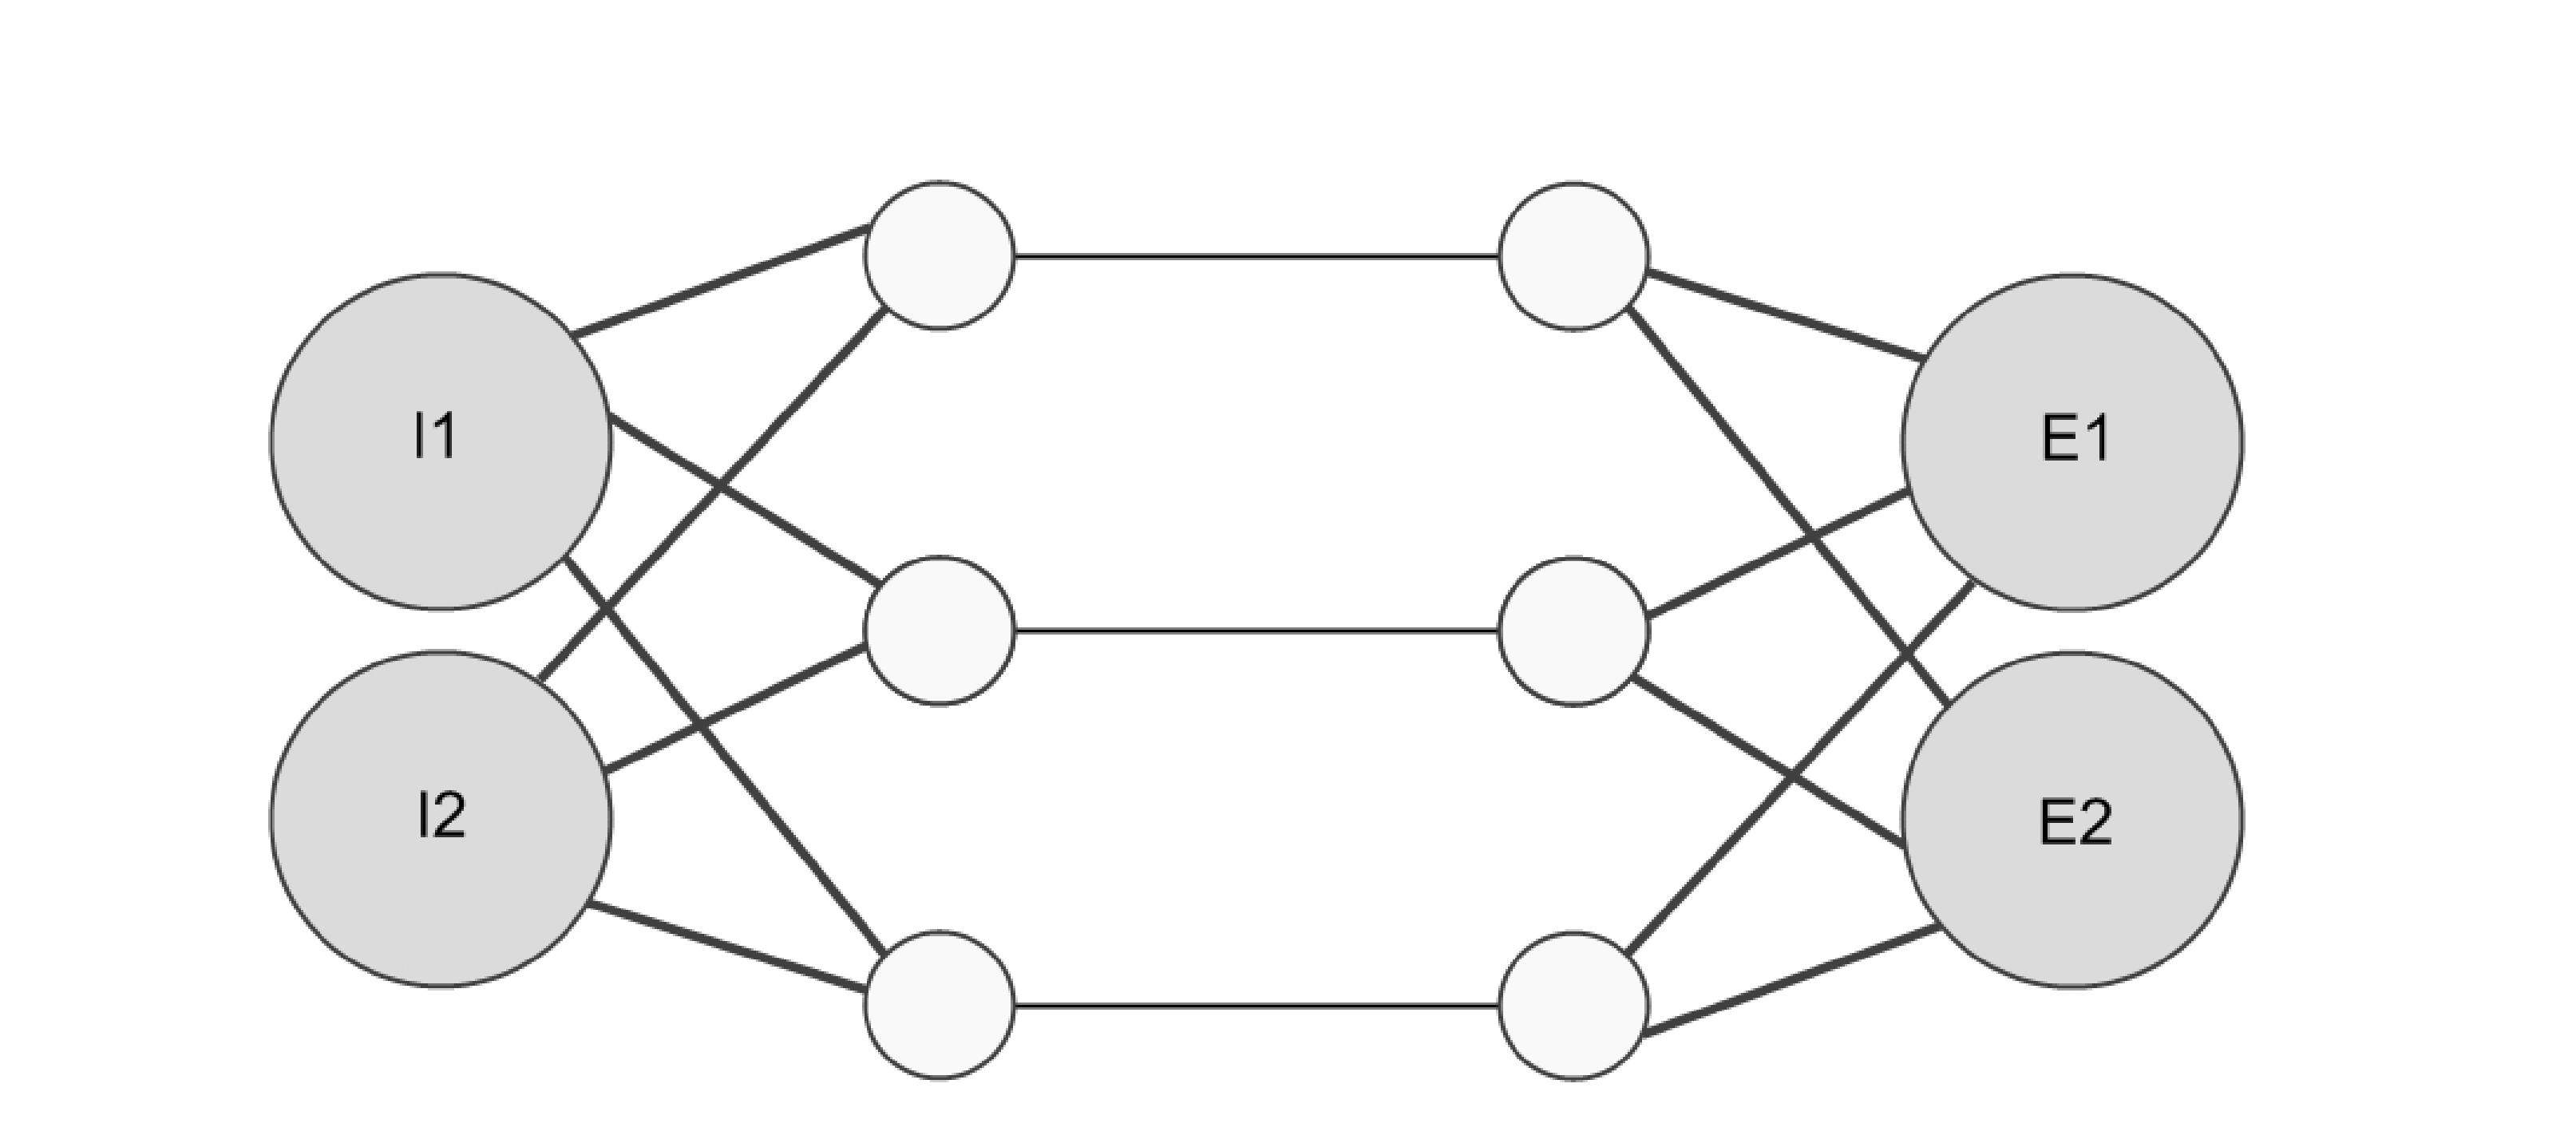
\epsfig{file=img/results/Topo232, width=4.5in}
\caption{
 Simulation topology for PREF analysis. 
 \label{fig:fwnd}
}
\end{center}
\end{figure}

Links have equal capacities and both  ingress points serve the same number of flows. The number of lows are equal during the first 300 sec, then the traffic demand changes and the number of flows to  E1 is doubled.

\subsection{Equalization Mode}

In this mode each balancer defines an equal split over the three paths for each of the destination. Figure \ref{fig:fwnd} illustrates the split for I1/E1. 

\begin{figure}[h!]
 \begin{center}
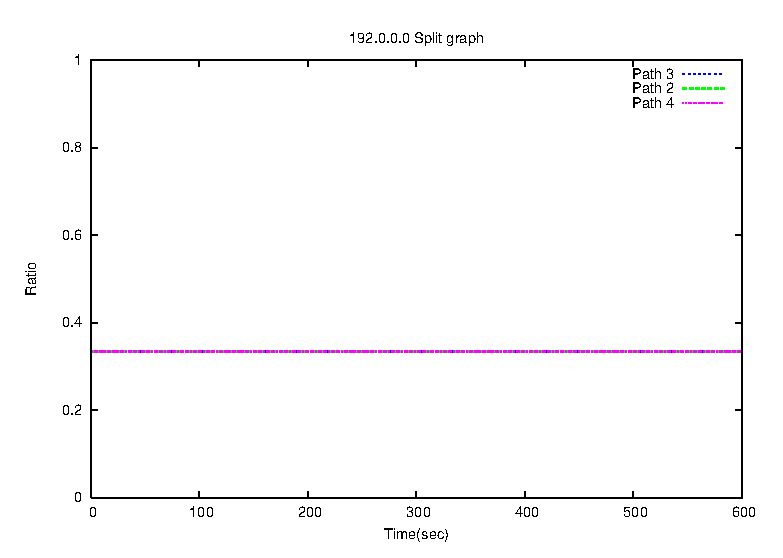
\epsfig{file=img/results/fwnd-192-0-0-0, width=4.5in}
\caption{
 Flowlet ratio $f_{i}$ for destination $E_{1}$ as set by ingress point $I_{1}$.
   \label{fig:fwnd}
}
\end{center}
\end{figure}

Figure \ref{fig:equal-thro-pref} shows that the throughputs over the different interfaces with PREF are not exactly the same as is the case for FLARE \ref{fig:equal-thro-flare}.  This is an expected result for PREF, since end host flows are composed from only one flowlet.  This means PREF is acting like a flow-based splitter. 
As such, the actual traffic splitting deviates from the desired split. On the other hand, FLARE achieves a good accuracy with the FLARE time out, the interval after which network associates a new path to a flow is set to 50ms, slightly larger then the maximum queueing time in the topology (approx 30ms) that corresponds to the time risk window when packet reordering could happen. We also observe that the throughputs obtained with PREF oscillate.

\begin{figure}[ht]
\centering
\subfigure[]{
  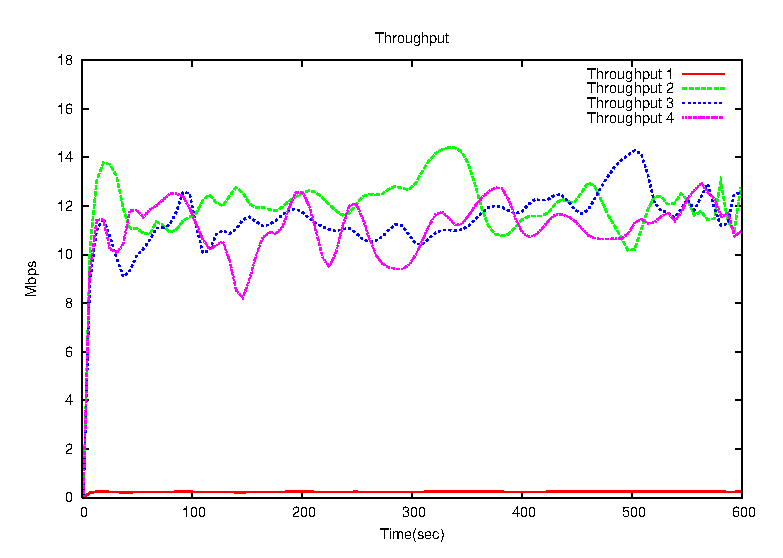
\includegraphics[scale=1]{img/results/pref/prefTput}
   \label{fig:equal-thro-pref}
}
\subfigure[]{
  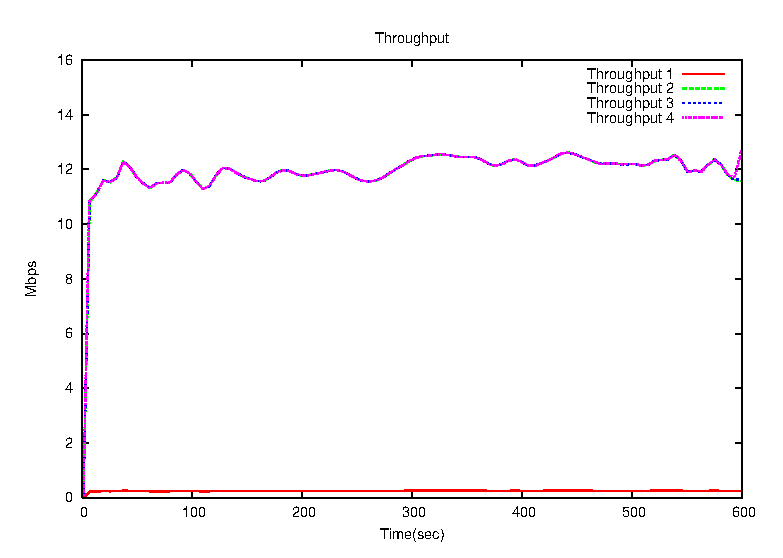
\includegraphics[scale=1]{img/results/pref/flareTput}
  \label{fig:equal-thro-flare}
}
\label{fig:throughputComparison}
\caption{Throughput of outgoing interfaces of I1 in equalization mode using \subref{fig:equal-thro-pref} PREF and \subref{fig:equal-thro-flare} FLARE.}
\end{figure}



\begin{figure}[ht]
\centering
\subfigure[]{
  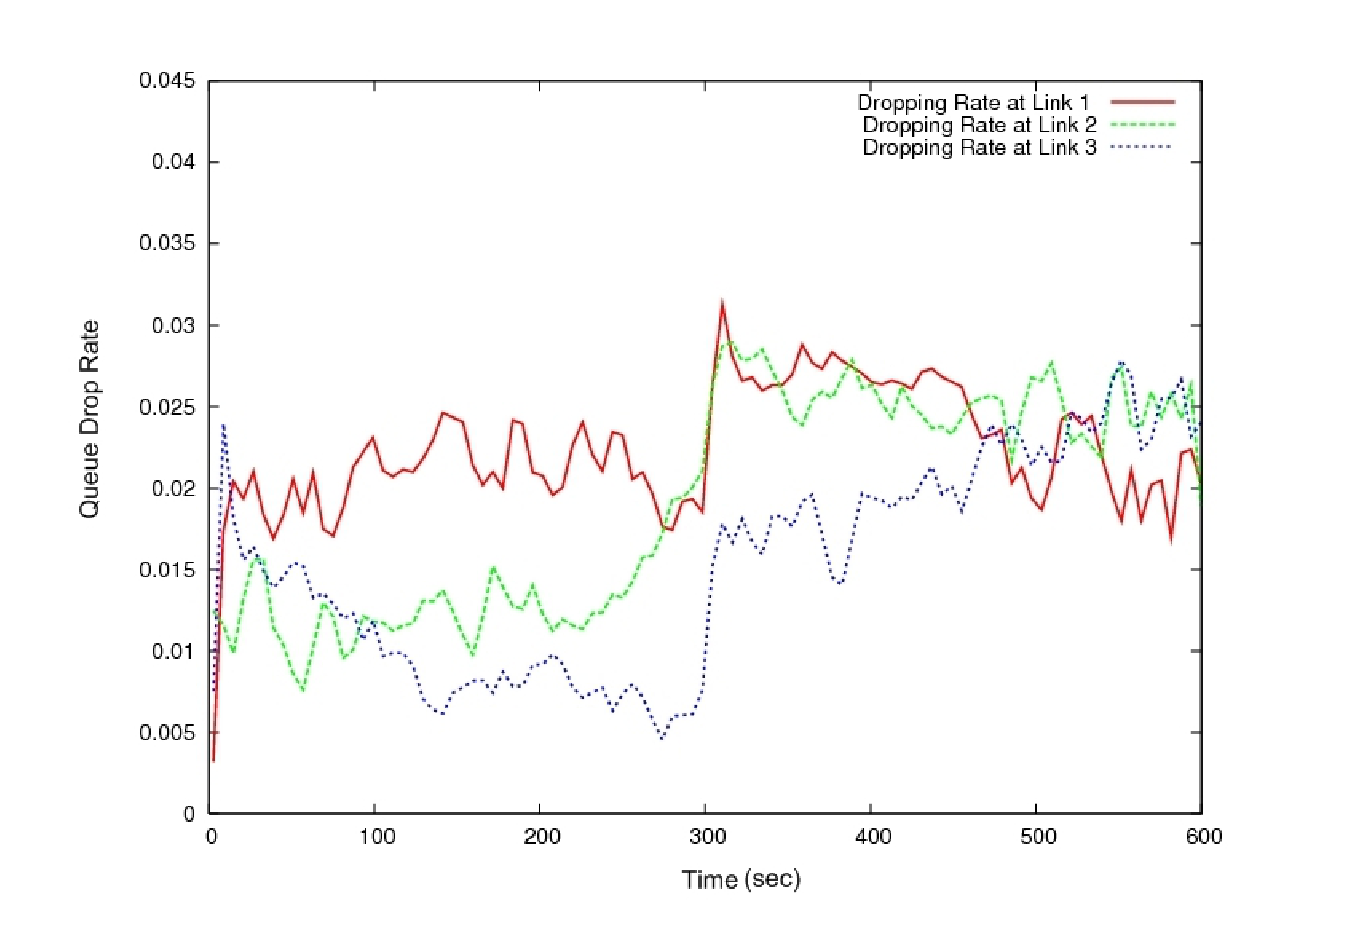
\includegraphics[width=5in]{img/results/pref/prefDrop}
   \label{fig:equal-drop-pref}
}
\subfigure[]{
  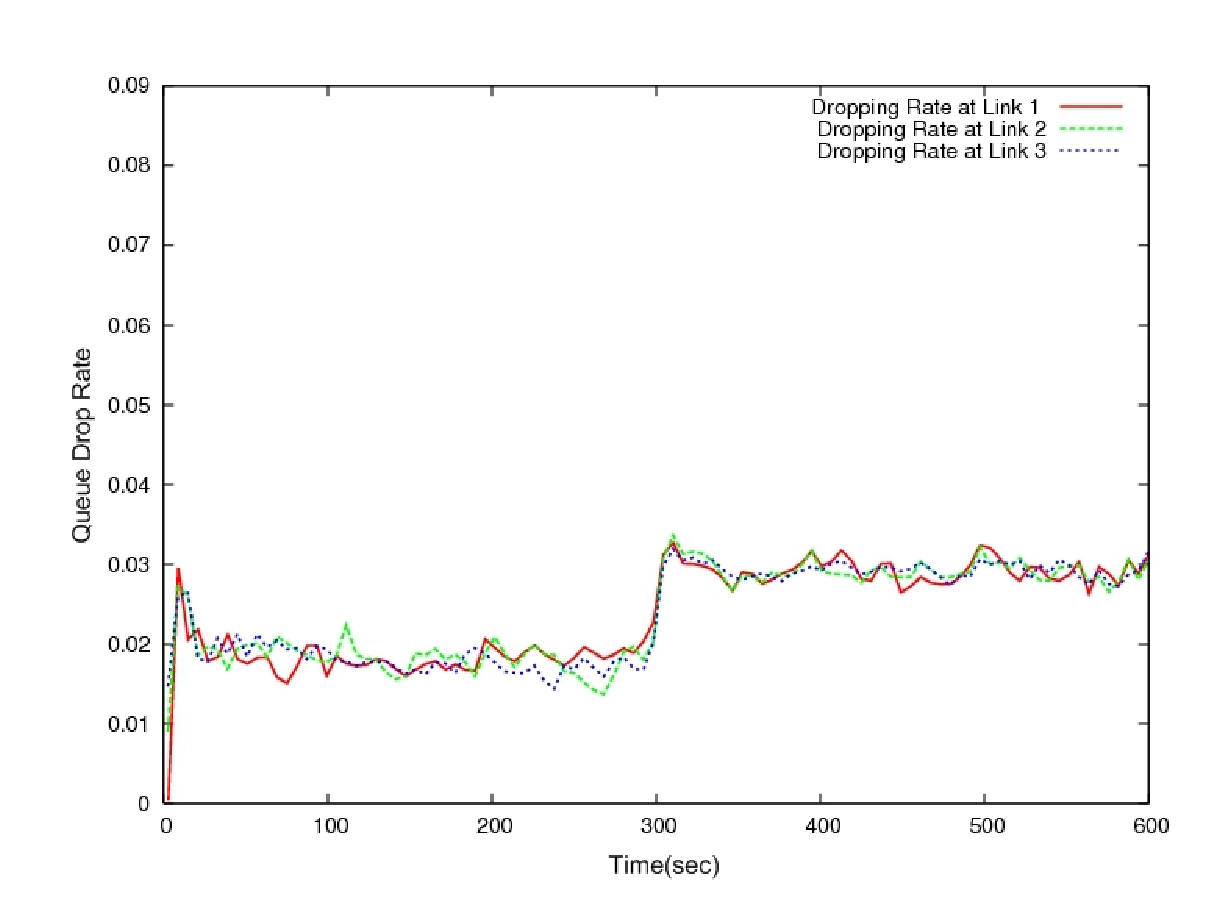
\includegraphics[width=5in]{img/results/pref/flareDrop}
  \label{fig:equal-drop-flare}
}
\label{fig:dropComparison}
\caption{Drop rate at bottlenecks in equalization mode using \subref{fig:equal-drop-pref} PREF and \subref{fig:equal-drop-flare} FLARE.}
\end{figure}


The unstable result obtained with PREF is confirmed with the drop rate observed at the bottlenecks  (figure \ref{fig:equal-drop-pref}), while a stable behaviour is observed for FLARE (figure \ref{fig:equal-drop-pref}). In fact,   network flowlets used by FLARE have a smaller order of granularity what make that the transport flows get a path attributed every few RTTs. As a result, the congestion level seen by a TCP routine is a combination of the congestion in the different paths and hence the flows adapt their transmission rate to a common level of congestion and the fluctuations are less significant  This is different than the path assignment process of PREF that makes the flowlets accommodate their  transmission rate to a single path.

\subsection{Balancing by path utilization}

The second example is  balancing by path utilization, a simplified version of TEXCP. The analysis from the previous example is still valid. Using PREF(figure \ref{fig:texcp-util-pref}), path utilization in the different paths is not as well balanced as it is with FLARE (figure \ref{fig:texcp-util-flare}). Yet, path utilization obtained is till good for the three links. 


\begin{figure}[h]
\centering
\subfigure[]{
  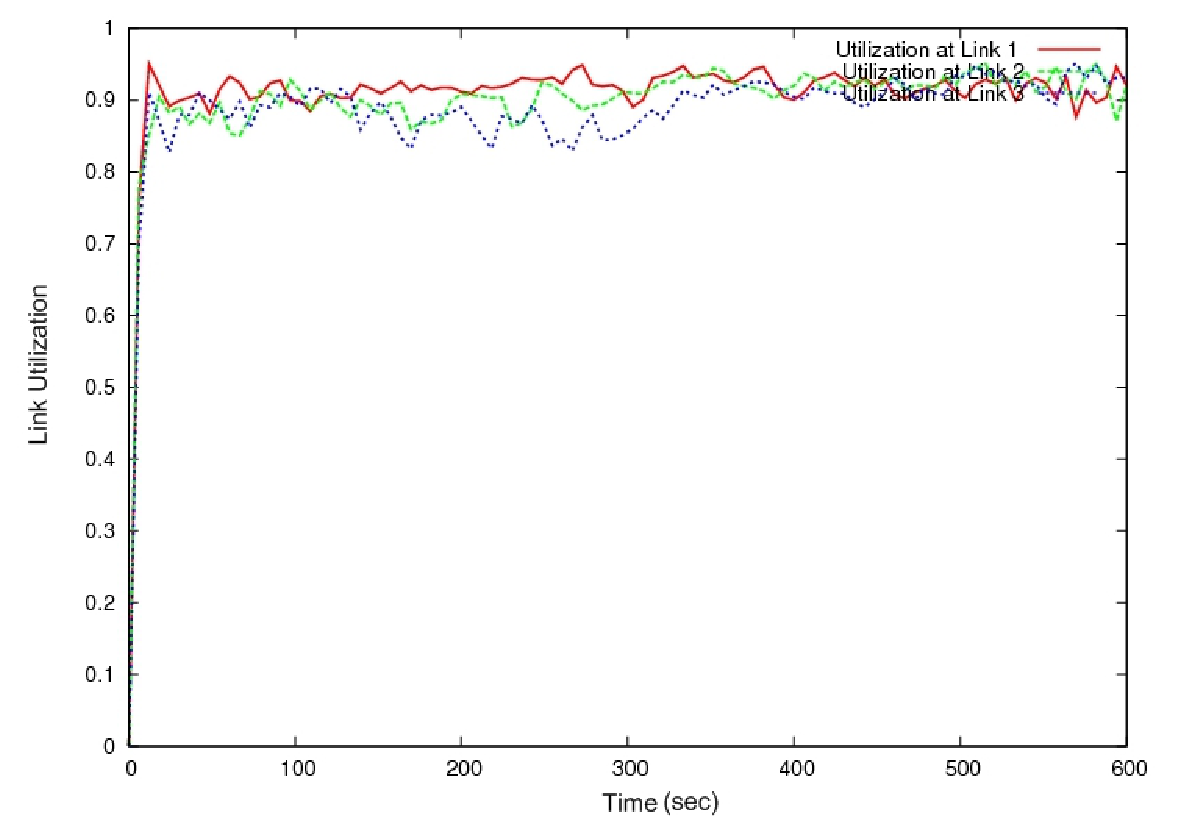
\includegraphics[width=5in]{img/results/sec5-1/equalization-PREF/util}
   \label{fig:texcp-util-pref}
}
\subfigure[]{
  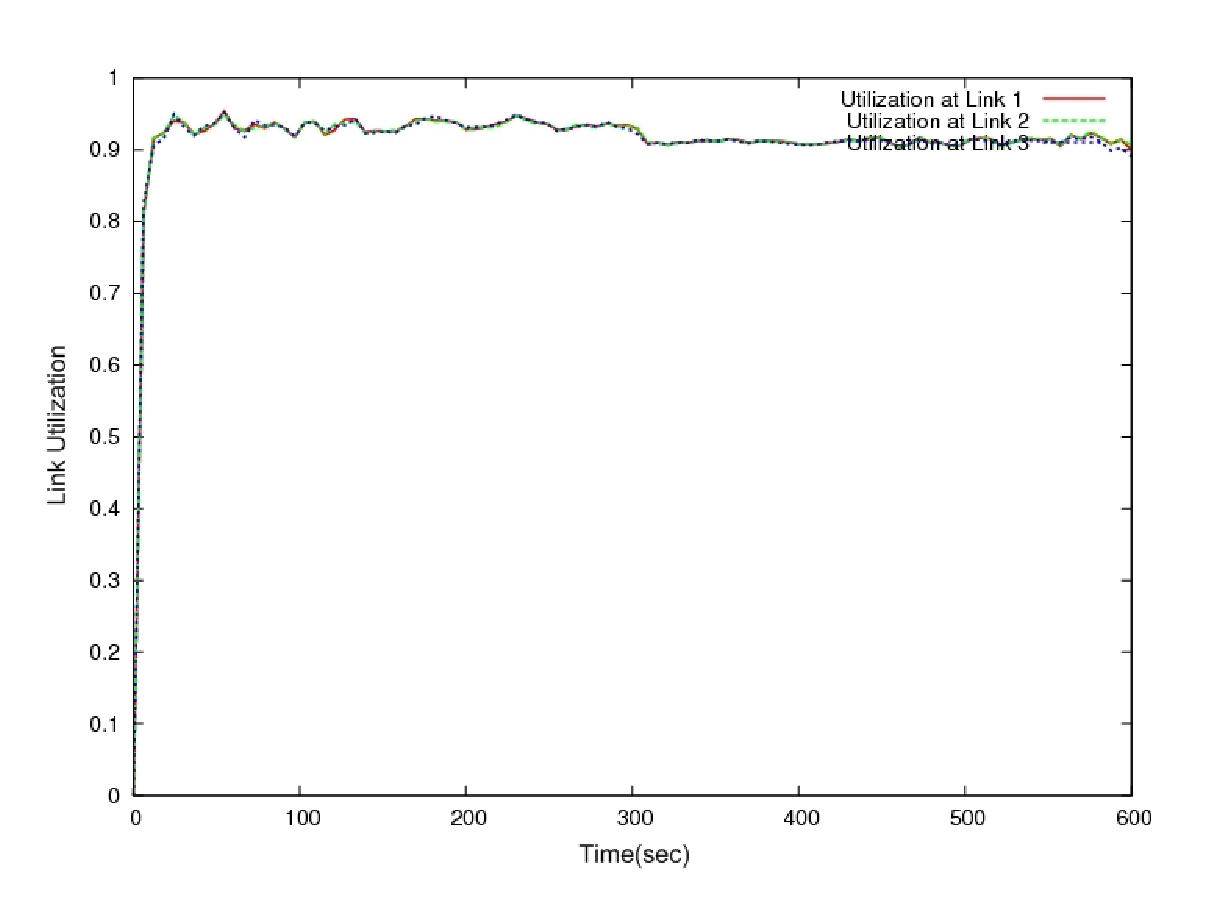
\includegraphics[width=5in]{img/results/sec5-1/texcp-flare/util}
  \label{fig:texcp-util-flare}
}
\label{fig:texcpComparison}
\caption{Path utilization measured at bottlenecks in Utilization Balancing mode using \subref{fig:texcp-util-pref} PREF and \subref{fig:texcp-util-flare} FLARE.}
\end{figure}


Using PREF for traffic splitting make balancing harder in classical load balancing approaches. From one hand, the obtained split deviates from the desired split. It also introduces more fluctuations compared with FLARE that makes the flows experience different paths and introduce a multiplexing effect that reduce fluctuation. Yet, PREF allows multiple architectural advantages to be achieved. It is important to mention that if end hosts apply more sophistical strategies on when and how often they request new paths, PREF performance will be significantly enhanced. 

